\section{Implementation}

\subsection{Description}

The main objective of this thesis has been to develop a solution that would notify users of data access events logged in the \textit{Andmejälgija} (Data Tracker) system. The resulting solution provides near real-time notifications when government institutions or other authorized entities access an eID holder's personal data.

\subsection{Discussion of implementation choice}
There are several possible approaches for developing such a solution. In this section I will discuss different implementation options as well as their advantages and disadvantages.

\subsubsection{X-Road service}
\textit{Andmejälgija} specifications require entities responsible for the state databases to implement an X-Road interface themselves, as described in \ref{protocol_desc}, so one option would be to create an X-Road service that would query \textit{Andmejälgija} data over X-Road directly from those entities. The main advantage of this approach would be the freedom in how to notify users of changes to the access logs. The service could support various communication channels, including instant messenger bots, e-mail and others. However, the list of requirements to operate such a service is daunting. 

\begin{itemize}
    \item {In order to join X-Road, legal entity is needed.}
    \item {Permission has to be requested from every X-Road service you want to query data from. Specifically, considering that each information system is responsible for implementing the \textit{Andmejälgija} protocol themselves, the permission would be required from each entity responsible for the information systems from which the access logs would be requested.}
    \item {As part of X-Road network, you need to operate a Security Server. It can be self-hosted anywhere for testing, but for production you need to have a Hardware Security Module (HSM), in order to be compliant with eIDAS requirements. For example, a Thales Luna PCIe HSM A700 suitable for eIDAS qualified digital signing costs €8,990 (€10,877.90 incl. VAT) \cite{thales-luna-hsm-pricing}. Alternatively, renting a production ready Security server from Telia costs 210€ per month \cite{telia-xroad-server}}
    \item {Finally, considering that this approach would include creating a service that would store and transmit user's data, it would be required to follow strict regulatory requirements including GDPR. Staying compliant requires a continuous effort, and in case of failure to do so, there are harsh fines.}
\end{itemize}

Satisfying this criteria is difficult and expensive. Additionally, even if I succeeded, people would have to consent and entrust me with their data in order to be able to use the solution, which is not in the spirit of creating a solution for monitoring personal data access as another data controller would be introduced.

\subsubsection{Standalone approach}
This approach uses the \textit{eesti.ee} session for accessing \textit{Andmejälgija} data. Once the user is logged in to the \textit{eesti.ee} state portal, certain internal API endpoints become available. Namely the \texttt{GET} endpoint \texttt{https://www.eesti.ee/\\andmejalgija/api/v1/usages} can be used to query \textit{Andmejälgija} data. The endpoint requires a parameter \texttt{dataSystemCodes} with which specific databases can be specified. For example, the GET request \texttt{/usages?dataSystemCodes=digiregistratuur\&\\dataSystemCodes=rahvastikuregister} would request access logs from \textit{Digiregistratuur} and \textit{Rahvastikuregister}.

The main advantage of this approach is the absence of all disadvantages of the X-Road approach: there is no need for any kind of bureaucracy and the solution could be an open-source project, available for anybody to compile and use. There arises a problem, however. What about the notification part? Do I expect users to set everything up on their hardware, including relevant communication channels? That would narrow down the project's user base to technical people knowing how to self-host, and having a server.

That's why I thought that creating a mobile application would be the most optimal approach. A mobile application would keep the \textit{eesti.ee} session alive and poll the \textit{Andmejälgija} API. This approach combines ease of setup and use while keeping the solution standalone, without requiring a central server.

\subsection{Development}

First, I had to determine how feasible and reliable the standalone approach would be, especially as I was dealing with a user-facing service that I would have to effectively reverse-engineer. The main challenge was to keep the session alive for as long as possible.

The \textit{eesti.ee} session is established using one of the strong authentication methods via the \textit{TARA} (Trusted Authentication and Authorization) service. Once the user is authenticated using ID-card, Mobile-ID, Smart-ID, or eID solution of another EU country, a JWT token is issued, valid for 30 minutes. The session management is then handled by \textit{GovSSO} (Government Single Sign-On), which maintains the master server-side session token and imposes certain limitations as discussed in \ref{session-limitations}.

Once the user is authenticated, certain internal API endpoints become available, including those for refreshing the JWT token and getting \textit{Andmejälgija} access logs. The JWT refresh endpoint returns Set-Cookie headers that include an updated JWTTOKEN on success, with an updated expiration date (30 minutes from the moment of extension).

To test whether the session could be kept alive indefinitely, I used the Tab Reloader extension for Firefox by James Fray \cite{tab-reloader-addon}. Using this browser extension, I configured the browser to automatically reload the tab with the JWT token refresh endpoint. After an 8-hour experiment, I deemed the approach successful.

The next step was the development of the \textbf{Data Access Notifier} Android application. I chose to develop it using the Kotlin programming language due to it being the new standard for developing Android applications \cite{kotlin-first}, as well as its more expressive syntax and promise of faster development speed.

The application is compatible with all Android versions starting from Android 8.1, meaning that it works on approximately 96.4\% of Android devices according to the Android Studio API version distribution chart \cite{android-api-distribution,android-studio-screenshot}.

\begin{figure}[H]
\centering
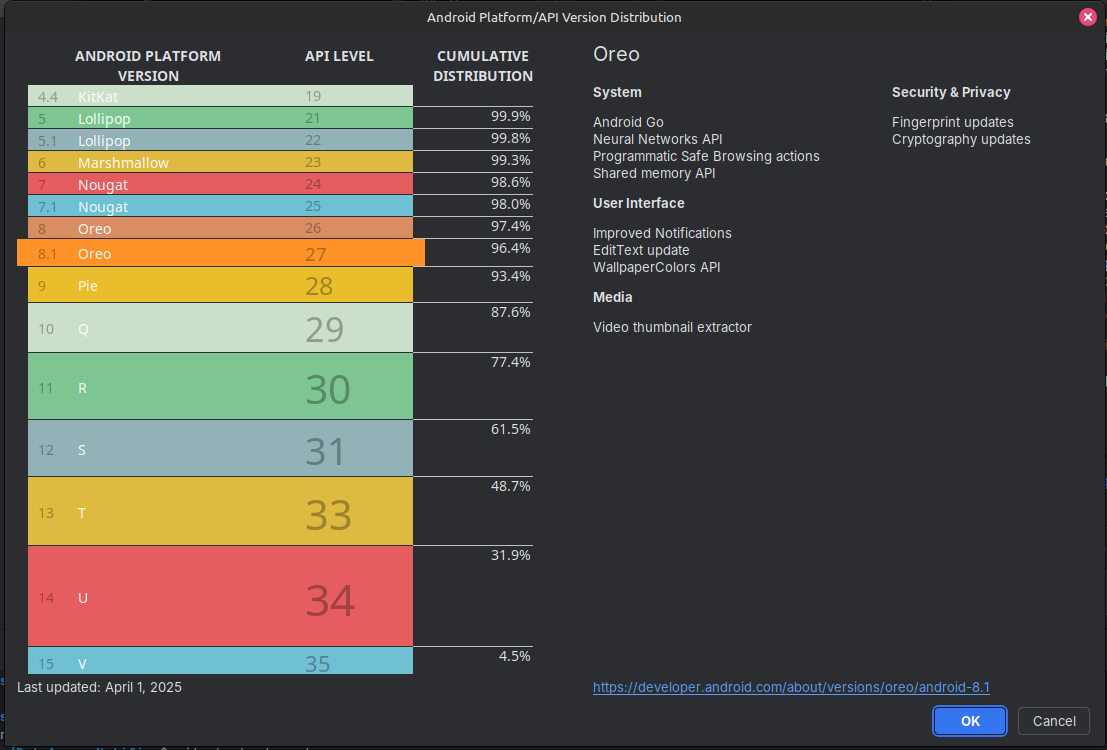
\includegraphics[width=450px]{english/figures/Screenshot from 2025-08-04 19-37-39.png}
\caption{Android Studio API Level Distribution showing compatibility percentages for different Android versions. The chart indicates that Android 8.1 (API level 27) and higher covers approximately 96.4\% of active devices.}
\label{fig:android-api-distribution}
\end{figure}

The software is open-source, licensed under the MIT license.

Currently, the application support is limited to Android 8.1 and higher. While support for iOS and other platforms is not planned due to limited development time and resources, anybody who deems this solution useful is encouraged to port it to platforms other than Android

\subsubsection{Authentication}
To gain access to \textit{eesti.ee} internal APIs, the user needs to be authenticated via \textit{TARA}. My initial plan was to reverse engineer the authentication flow and authenticate the user by sending raw HTTP requests and returning responses. This approach, however, would be fragile and require substantial engineering effort to develop and maintain.

Instead, I decided to use Android WebView for authentication as a more reliable and convenient approach for both the user and the developer. By leveraging WebView, the \textbf{Data Access Notifier} application can present the official \textit{TARA} login page directly to the user, allowing them to authenticate using their preferred method (ID-card, Mobile-ID, Smart-ID, or eID of another EU country). This approach significantly reduces the risk of breaking changes due to updates on the \textit{eesti.ee} or \textit{TARA} platforms. Once the user is authenticated, the application can access the necessary session cookies and JWT token to interact with the internal APIs.

\subsubsection{Interacting with \textit{eesti.ee} internal APIs}
For interacting with \textit{eesti.ee} internal APIs, I used the OkHttp library by Square, Inc. \cite{okhttp-library}. I utilized the following API endpoints:

\begin{itemize}
    \item \textbf{GET} \texttt{https://www.eesti.ee/timur/jwt/extend-jwt-session}
    
    An endpoint for extending JWT session.
    
    \item \textbf{GET} \texttt{https://www.eesti.ee/andmejalgija/api/v1/usages}
    
    An endpoint for querying Data Tracker access logs.
    
    Query parameters:
    \begin{itemize}
        \item \texttt{dataSystemCodes}: The name of the information system the access logs are queried from.
    \end{itemize}
    
    \samepage
    Response body format (JSON):
    \begin{small}
    \begin{verbatim}
{
  "findUsageResponses": [
    {
      "logTime": "2025-08-03T22:40:47",
      "receiver": "Tervise ja Heaolu Infosüsteemide Keskus",
      "infoSystemCode": "rahvastikuregister",
      "action": "ISIKU NIME VÄLJASTAMINE ISIKUKOODI PÕHJAL"
    },
    ...
  ]
}
    \end{verbatim}
    \end{small}
    
    Response fields:
    \begin{itemize}
        \item \texttt{logTime}: Timestamp of the data access event in ISO 8601 format
        \item \texttt{receiver}: Registry code of the entity that accessed the data
        \item \texttt{infoSystemCode}: Code identifying the information system
        \item \texttt{action}: Description of the action performed (in Estonian)
    \end{itemize}
\end{itemize}

Both endpoints require a valid JWT token to succeed. WebView's CookieManager serves as a single source of truth in this application, where all cookies are loaded from for making requests and written to upon receiving responses.

\subsubsection{Keeping the session alive}
The API requests are authenticated using a JWT token cookie, the lifetime of which is 30 minutes. This means that the \textbf{Data Access Notifier} application must either run a continuous foreground service or be awakened periodically to request an updated JWT token and send requests to \textit{Andmejälgija}.

On Android, there are several ways to accomplish this, although it is worth mentioning that Android is very restrictive regarding background tasks and battery usage. I tried several approaches and will describe my experience with them in the context of developing this application.

\subsubsection{WorkManager approach}
According to the Android documentation, WorkManager is the recommended solution for persistent work. Work is persistent when it remains scheduled through app restarts and system reboots. This seemed to describe my use case very well, so this was the first approach that I tried.

Work is defined in WorkManager using a WorkRequest. There are several WorkRequest types available, including PeriodicWorkRequest and OneTimeWorkRequest.

Using PeriodicWorkRequest, it is possible to schedule periodic tasks. The important limitation here is that it is not possible to schedule a task to execute more frequently than every 15 minutes. While this may sound appropriate for the use case of having to renew the session at least every 30 minutes, in practice, the situation is different.

During development, I discovered a critical difference between session handling in web browsers versus HTTP client libraries. While the browser-based testing with Tab Reloader successfully maintained the session by refreshing the JWT token every 15 minutes, the same approach using OkHttp in the Android application failed to keep the session alive.

The exact cause of this discrepancy remains unclear. It appears that the \textit{eesti.ee} session management system expects more frequent interaction or handles cookie management differently when requests originate from HTTP client libraries compared to full web browsers. Indeed, with shorter intervals of 5 minutes, the session remains alive. This behavioral difference rendered the PeriodicWorkRequest approach with 15-minute intervals unsuitable for maintaining persistent sessions in the application context.

While OneTimeWorkRequest is designed for one-time tasks, it is possible to chain them by having each one-time work create another one-time work at the end of its lifespan. This approach allows setting custom intervals shorter than 15 minutes, circumventing the limitation imposed by PeriodicWorkRequest.

While OneTimeWorkRequest may appear to be a suitable solution, WorkManager itself proved to be rather unreliable for my use case after testing. The limitation of WorkManager is that tasks scheduled by it are managed by the system and may be deferred if deemed necessary by the Android system. For example tasks may not execute if the phone has low battery level, or even in other scenarios depending on the aggressiveness of the Android variant regarding the restrictions imposed on application behavior.

\subsubsection{Foreground service approach}
A foreground service is one of the most reliable types of tasks an application can schedule. In contrast to background services, foreground services are considered to be of higher priority by the system and thus are not candidates for termination when the system is low on memory or the phone has low battery level.

However, an important limitation has been introduced in recent Android versions. More specifically, starting from Android 15, the system places restrictions on how long certain foreground services are allowed to run while the application is in the background. Currently, this restriction only applies to dataSync and mediaProcessing foreground service types. The foreground services of those types are allowed to run for a total of 6 hours in a 24-hour period \cite{android-15-datasync-timeout}.

The most appropriate foreground service type for my use case is dataSync, meaning that it falls under the 6-hour per day restriction. While it should be possible to choose an arbitrary foreground service type regardless of the actual task type, doing so is not the cleanest approach, especially considering the existence of better alternatives. Furthermore, doing so may also impact the application's acceptance into the Google Play Store.

\subsubsection{Hybrid AlarmManager approach}
\label{alarmmanager-approach}
After evaluating the limitations of WorkManager and the restrictions on foreground services, I ultimately settled on a hybrid approach combining AlarmManager with a dataSync foreground service. AlarmManager is a system service that allows scheduling operations to be executed at specific times, even if the application is not running. By using AlarmManager to trigger the application at regular intervals (e.g., every 5 minutes), it is ensured that the session renewal and data polling tasks are reliably executed.

When the alarm fires, the application starts a short-lived dataSync foreground service to perform the necessary network operations: refreshing the JWT token and querying the \textit{Andmejälgija} API. This approach leverages the reliability of foreground services for critical tasks while minimizing battery usage by only running the service when needed. AlarmManager itself is not subject to aggressive background restrictions and can wake the application even in Doze mode, making it suitable for periodic tasks.

This solution proved to be robust and reliable across different Android versions and device manufacturers. Both AlarmManager and foreground services are extremely reliable even under low battery conditions, ensuring that the session remains alive and notifications are delivered promptly to the user.

\subsubsection{Session limitations}
\label{session-limitations}
During the development and testing process, I discovered an important server-side limitation that affects the overall feasibility of the session-based approach. Despite the successful implementation of session renewal mechanisms, the \textit{GovSSO} session management system imposes a hard limit of 12 hours on session duration. After this period, the session expires permanently and cannot be renewed.

The problem was discovered when it became apparent that JWT extension fails regularly with response code 500 (Internal Server Error) from the server and no further information. Following a number of retries, the server would send code 400 (Bad Request). At some point I started looking for a pattern and discovered that the session extension starts failing after exactly 12 hours. I investigated the \textit{GovSSO} GitHub repository \cite{govsso-session} and found the answer in the configuration file.

In the file \texttt{/src/main/resources/application.yml}, the following configuration parameter is defined:

\begin{small}
\begin{verbatim}
session-max-duration-hours: 12
\end{verbatim}
\end{small}

The function responsible for checking the \texttt{notBefore} date of the JWT token is shown below \cite{govsso-session-hydra}:

\begin{small}
\begin{verbatim}
private boolean isNbfValid(JWT idToken) throws ParseException {
    Date idTokenDate = idToken.getJWTClaimsSet().getNotBeforeTime();
    Date currentDate = new Date();
    long diffInMillis = Math.abs(currentDate.getTime() -
                                        idTokenDate.getTime());
    long diffInSeconds = TimeUnit.SECONDS.convert(diffInMillis, 
                                        TimeUnit.MILLISECONDS);
    long maxDurationInSeconds = TimeUnit.SECONDS.convert(
        ssoConfigurationProperties.getSessionMaxDurationHours(), 
        TimeUnit.HOURS);

    return diffInSeconds <= maxDurationInSeconds;
}
\end{verbatim}
\end{small}

Initially, I hypothesized that this limitation was related to the JWT token issued to the client, with the server rejecting it once it reaches the age of 12 hours. This would have been an easy fix, as there is another way to extend the session that would issue a "fresh" JWT token each time. As can be derived from the name "\textit{GovSSO}", this authentication service supports single-sign-on, meaning that if you are signed into one state e-service, you can log into another by clicking a "Continue session" button. The same can be achieved for the same state portal where the system was initiated, if you go to the right URL. Automating this kind of flow is straightforward.

\begin{figure}[H]
\centering
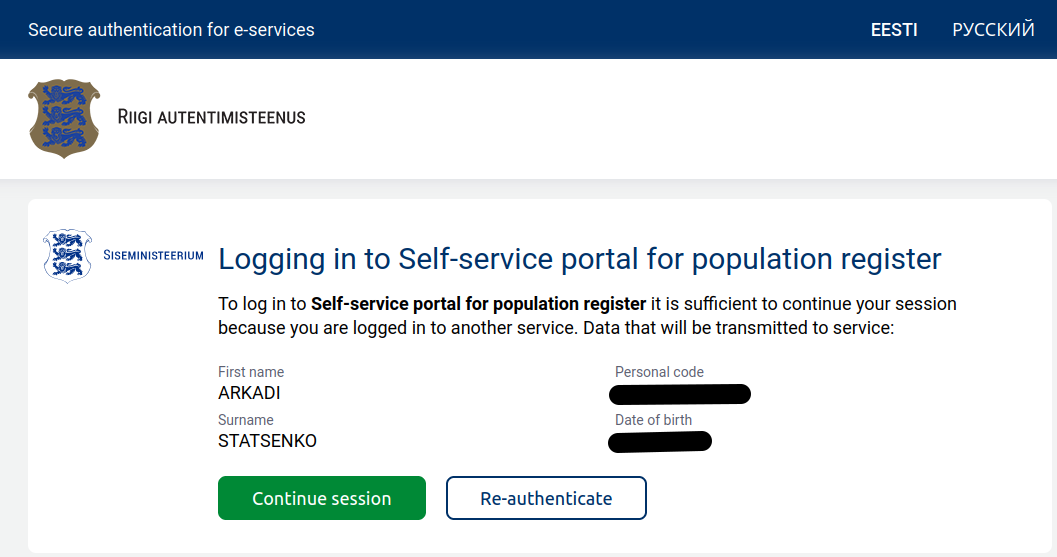
\includegraphics[width=450px]{english/figures/Screenshot from 2025-08-08 20-37-42.png}
\caption{A single sign-on interface showing the "Continue session" option that allows users to extend their authentication session across different government e-services \cite{eesti-ee-screenshot}.}
\label{fig:eesti-ee-continue-session}
\end{figure}

However, after experimenting with this method, I discovered that the 12-hour limitation applies to a different token than initially expected. The time validation is not performed on the client-side JWT token that the application receives, but rather on a server-side master JWT token that is created during the initial \textit{TARA} authentication process (ID-card, Mobile-ID, Smart-ID, etc.) and managed by \textit{GovSSO}.

When a user logs into additional services using the single-sign-on functionality, these secondary sessions are all linked to the same original server-side JWT token managed by \textit{GovSSO}. This architecture means that regardless of which session extension method is used, the 12-hour limit cannot be circumvented because all sessions share the same underlying authentication token that expires after 12 hours.

This limitation has significant implications for the notification system's reliability. Users who expect continuous monitoring must re-authenticate manually at least once every 12 hours to maintain the service functionality. However, this constraint is substantially mitigated by the API's design, which ensures that no data access events are permanently lost, though it does introduce periodic interruptions in real-time monitoring.

Specifically, the API returns comprehensive historical access logs, ensuring that once a user re-authenticates after a session expiry, they will receive all notifications for events that occurred during the period when they were logged out. This behavior is crucial for maintaining data completeness and ensuring that no critical access events are missed due to authentication gaps. The technical implementation of this log handling is detailed in \ref{log-handling}.

\subsubsection{Handling logs and notification delivery}
\label{log-handling}
In this section the following aspects of access log handling will be tackled: their storage, deduplication and filtering.

First of all, user inquiries about themselves are also considered data access and therefore produce access logs. This includes \textit{Andmejälgija} data queries. However, making frequent queries to the \textit{Andmejälgija} API produces a lot of logs. 

This makes it important to distinguish logs made by the user themselves from the logs made by third-parties. Thankfully, the \texttt{receiver} field contains the user's Estonian personal code in case the query is made by them. In fact, filtering by whether the receiver field contains user's personal code is exactly how the access log filtering is implemented on \textit{eesti.ee} itself when the user ticks the "Exclude queries I have made/initiated" checkbox. Here is the \textit{eesti.ee} code extract that demonstrates this approach \cite{eesti-ee-portal}:

\begin{small}
\begin{verbatim}
this.accountService.getUserInfo().subscribe((o) => {
    this.filteredData.data = this.filteredData.data.filter(
        (d) => !d.receiver.toUpperCase()
                   .includes(o.personalCode.replace(/^EE/, ""))
    );
})
\end{verbatim}
\end{small}

This is exactly how I implemented log filtering in the application. The user's personal code that is needed for filtering is extracted from the JWT token, along with the first name which is used to greet the user.

For deduplication of access logs, I utilized the Set data structure. Each access log entry is represented as a data class, and a Set of these entries is maintained to ensure that duplicate logs are not stored or processed multiple times. This approach leverages the fact that Sets in Kotlin do not allow duplicate elements.

To persist the access logs across app restarts and device reboots, I used Proto Data Store, which is Android's recommended solution for storing typed objects or lists in a transactional and type-safe manner. Proto Data Store uses Protocol Buffers \cite{protocol-buffers} for serialization, offering efficient storage and schema evolution capabilities.

Whenever new logs are fetched from the API, they are first filtered to exclude self-access events. The newly fetched logs are then merged with the existing logs stored in Proto Data Store, and the combined set is deduplicated using Kotlin's Set data structure. To determine which logs are new and should trigger notifications, the application computes the set difference between the combined deduplicated logs and the previously stored logs. Only the new items resulting from this difference are used to notify the user. This approach ensures that notifications are sent only for genuinely new access events, while avoiding redundant alerts for logs that have already been seen.

\subsection{Software distribution}

The \textbf{Data Access Notifier} application is distributed as an open-source project hosted on GitHub \cite{data-access-notifier}. Users can download the APK file directly from the GitHub Releases page \cite{data-access-notifier-releases}. To keep the application up to date, users can utilize third-party applications such as Obtainium \cite{obtainium}, which enables automatic updates for applications distributed outside of traditional app stores.

While the application is not currently available from app stores like Google Play Store, this possibility is not excluded in the future. Any updates regarding the application distribution would be posted on GitHub README.

\subsection{User guide}
After installation and opening for the first time, the \textbf{Data Access Notifier} application will prompt user for necessary permissions, which are the ability to schedule alarms (for AlarmManager to work) as well as to post notifications.

Once the necessary permissions are given, the Log In screen appears. When Log In button is pressed, an Android WebView is opened, redirecting the user to \textit{TARA} Log In screen. There user is free to choose whatever state authentication option they choose.

And that's it! As soon as authentication is successfully completed, you will start receiving notifications as soon as there are any new data access logs returned from the server. There is also a view inside of the application showing all data access logs saved.

\begin{figure}[H]
\centering
\begin{minipage}{0.32\textwidth}
    \centering
    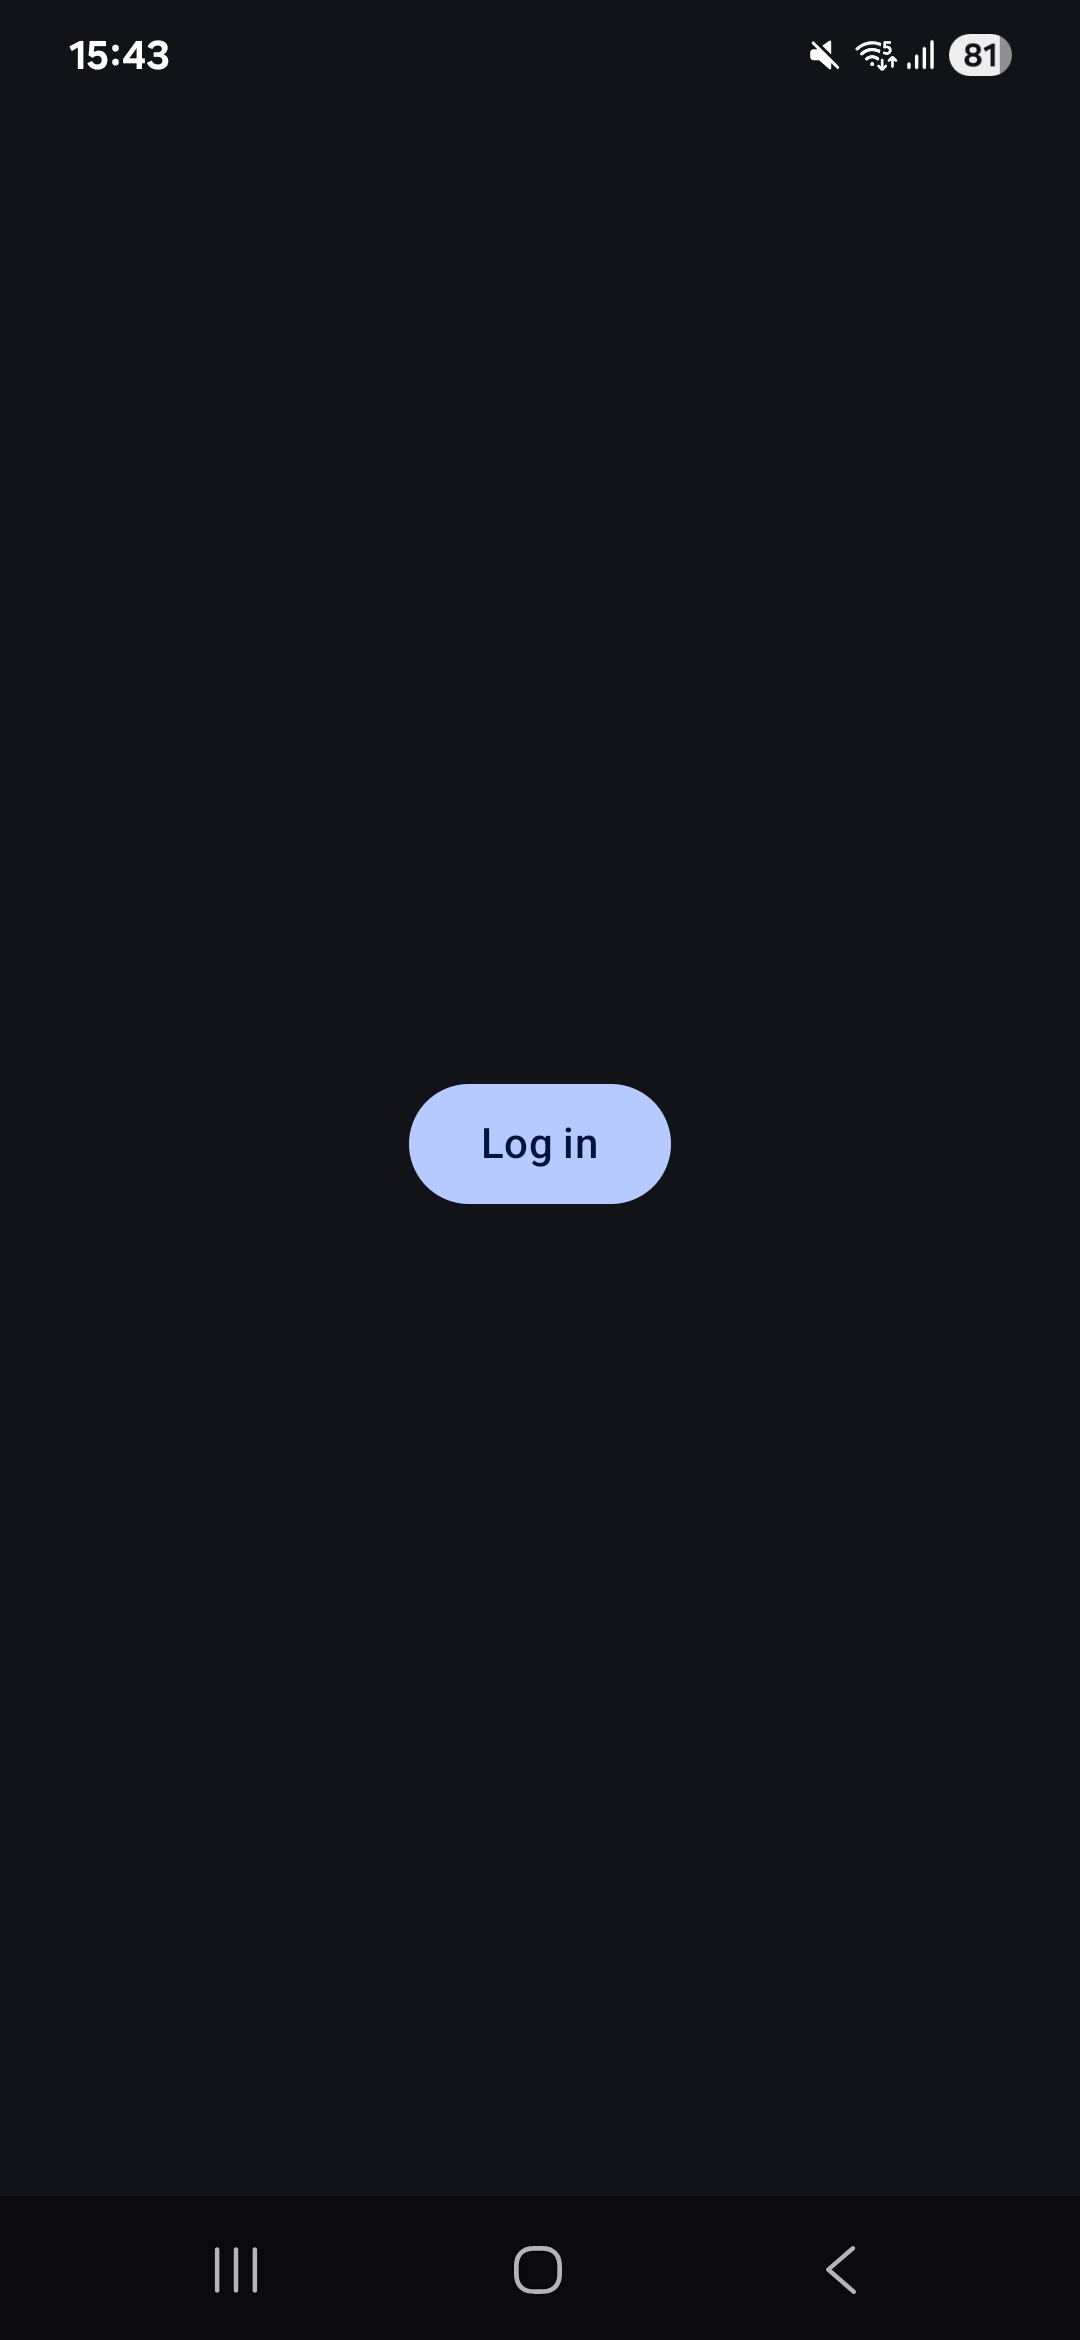
\includegraphics[width=\textwidth]{english/figures/Screenshot_20250810_154333_Data Access Notifier.jpg}
\end{minipage}%
\hfill
\begin{minipage}{0.32\textwidth}
    \centering
    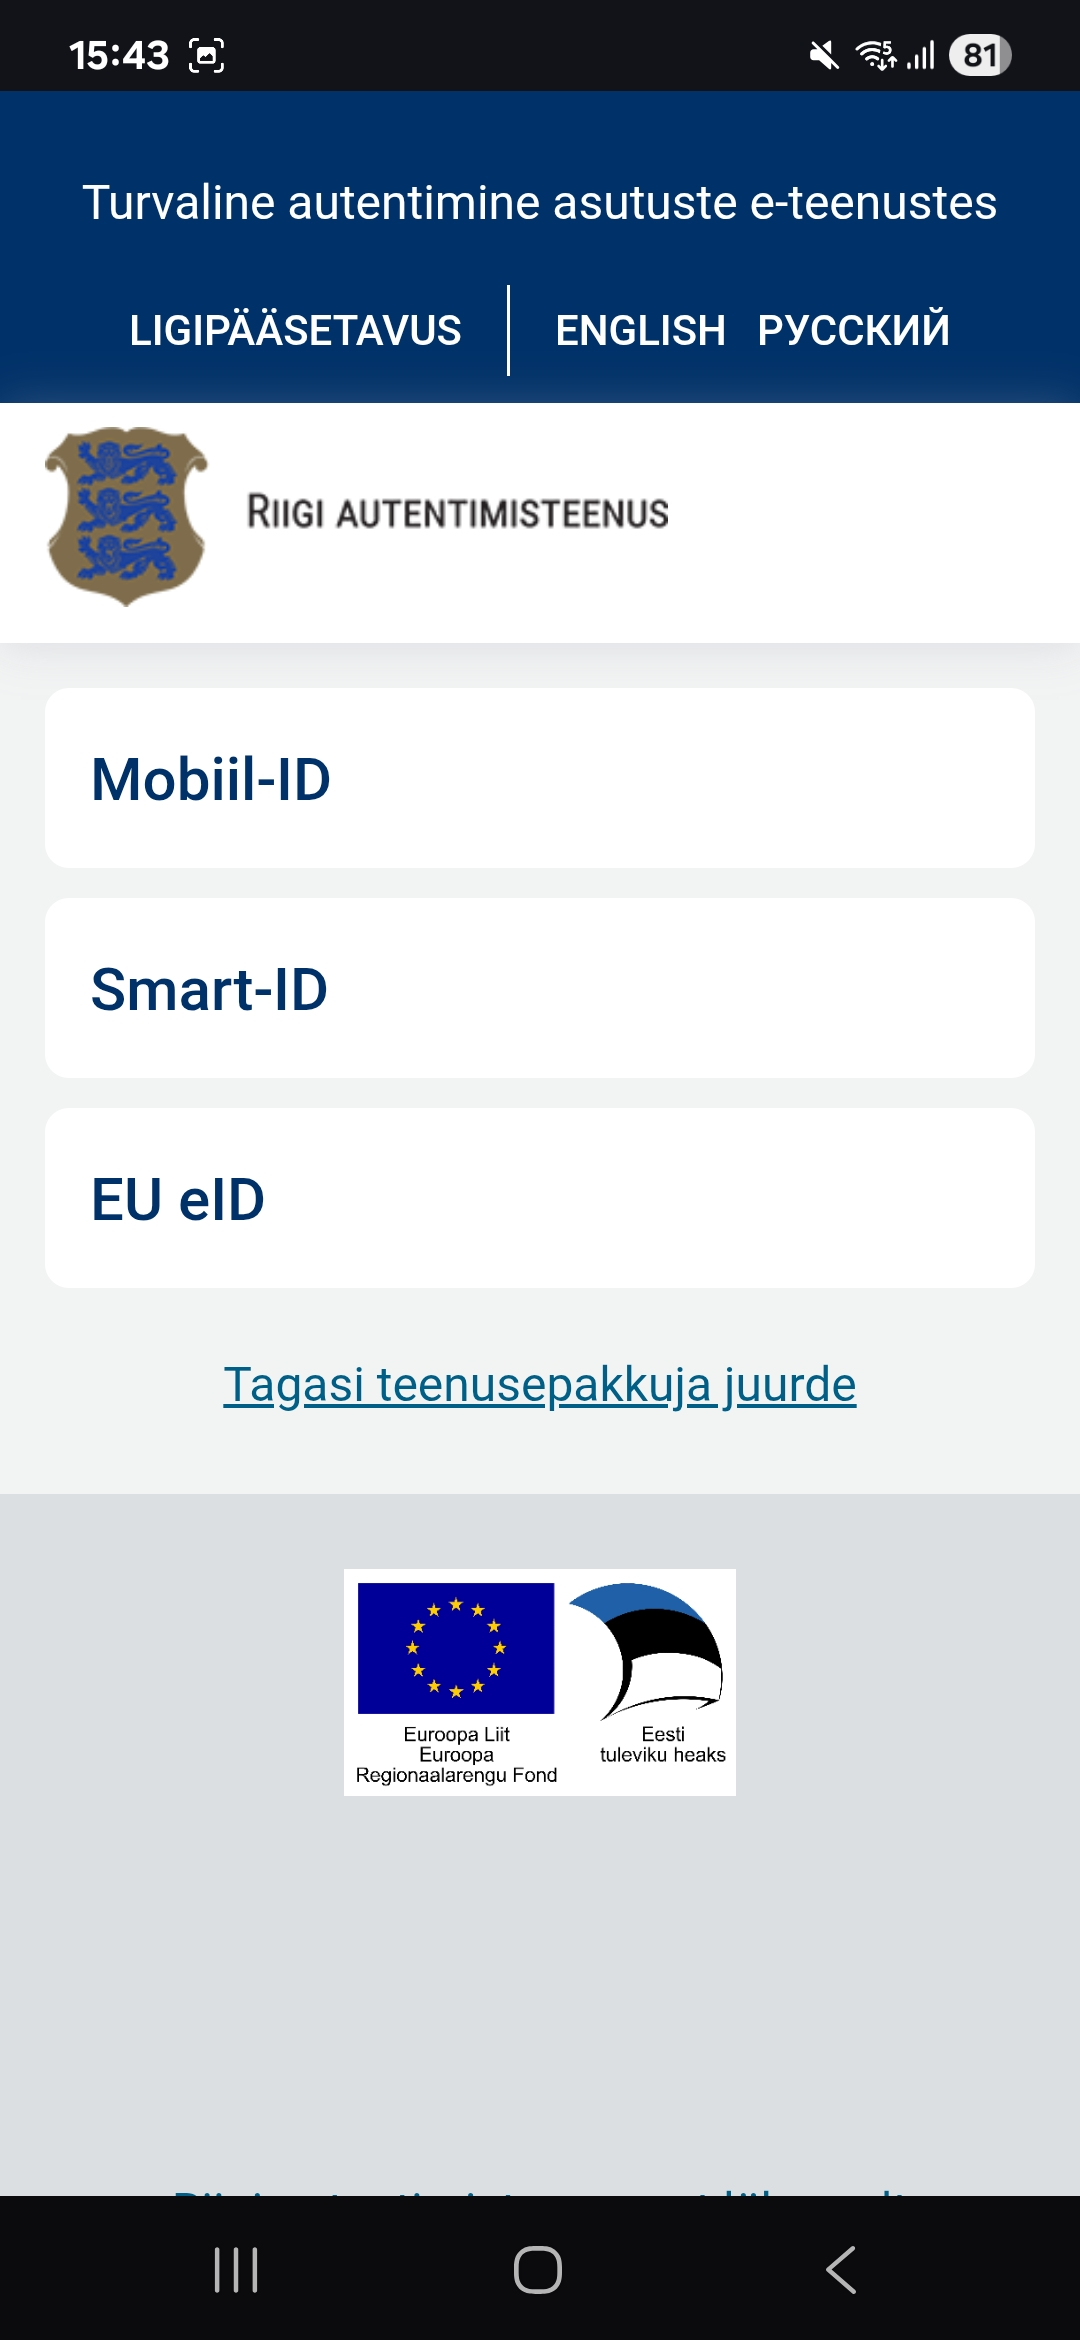
\includegraphics[width=\textwidth]{english/figures/Screenshot_20250810_154342_Data Access Notifier.jpg}
\end{minipage}%
\hfill
\begin{minipage}{0.32\textwidth}
    \centering
    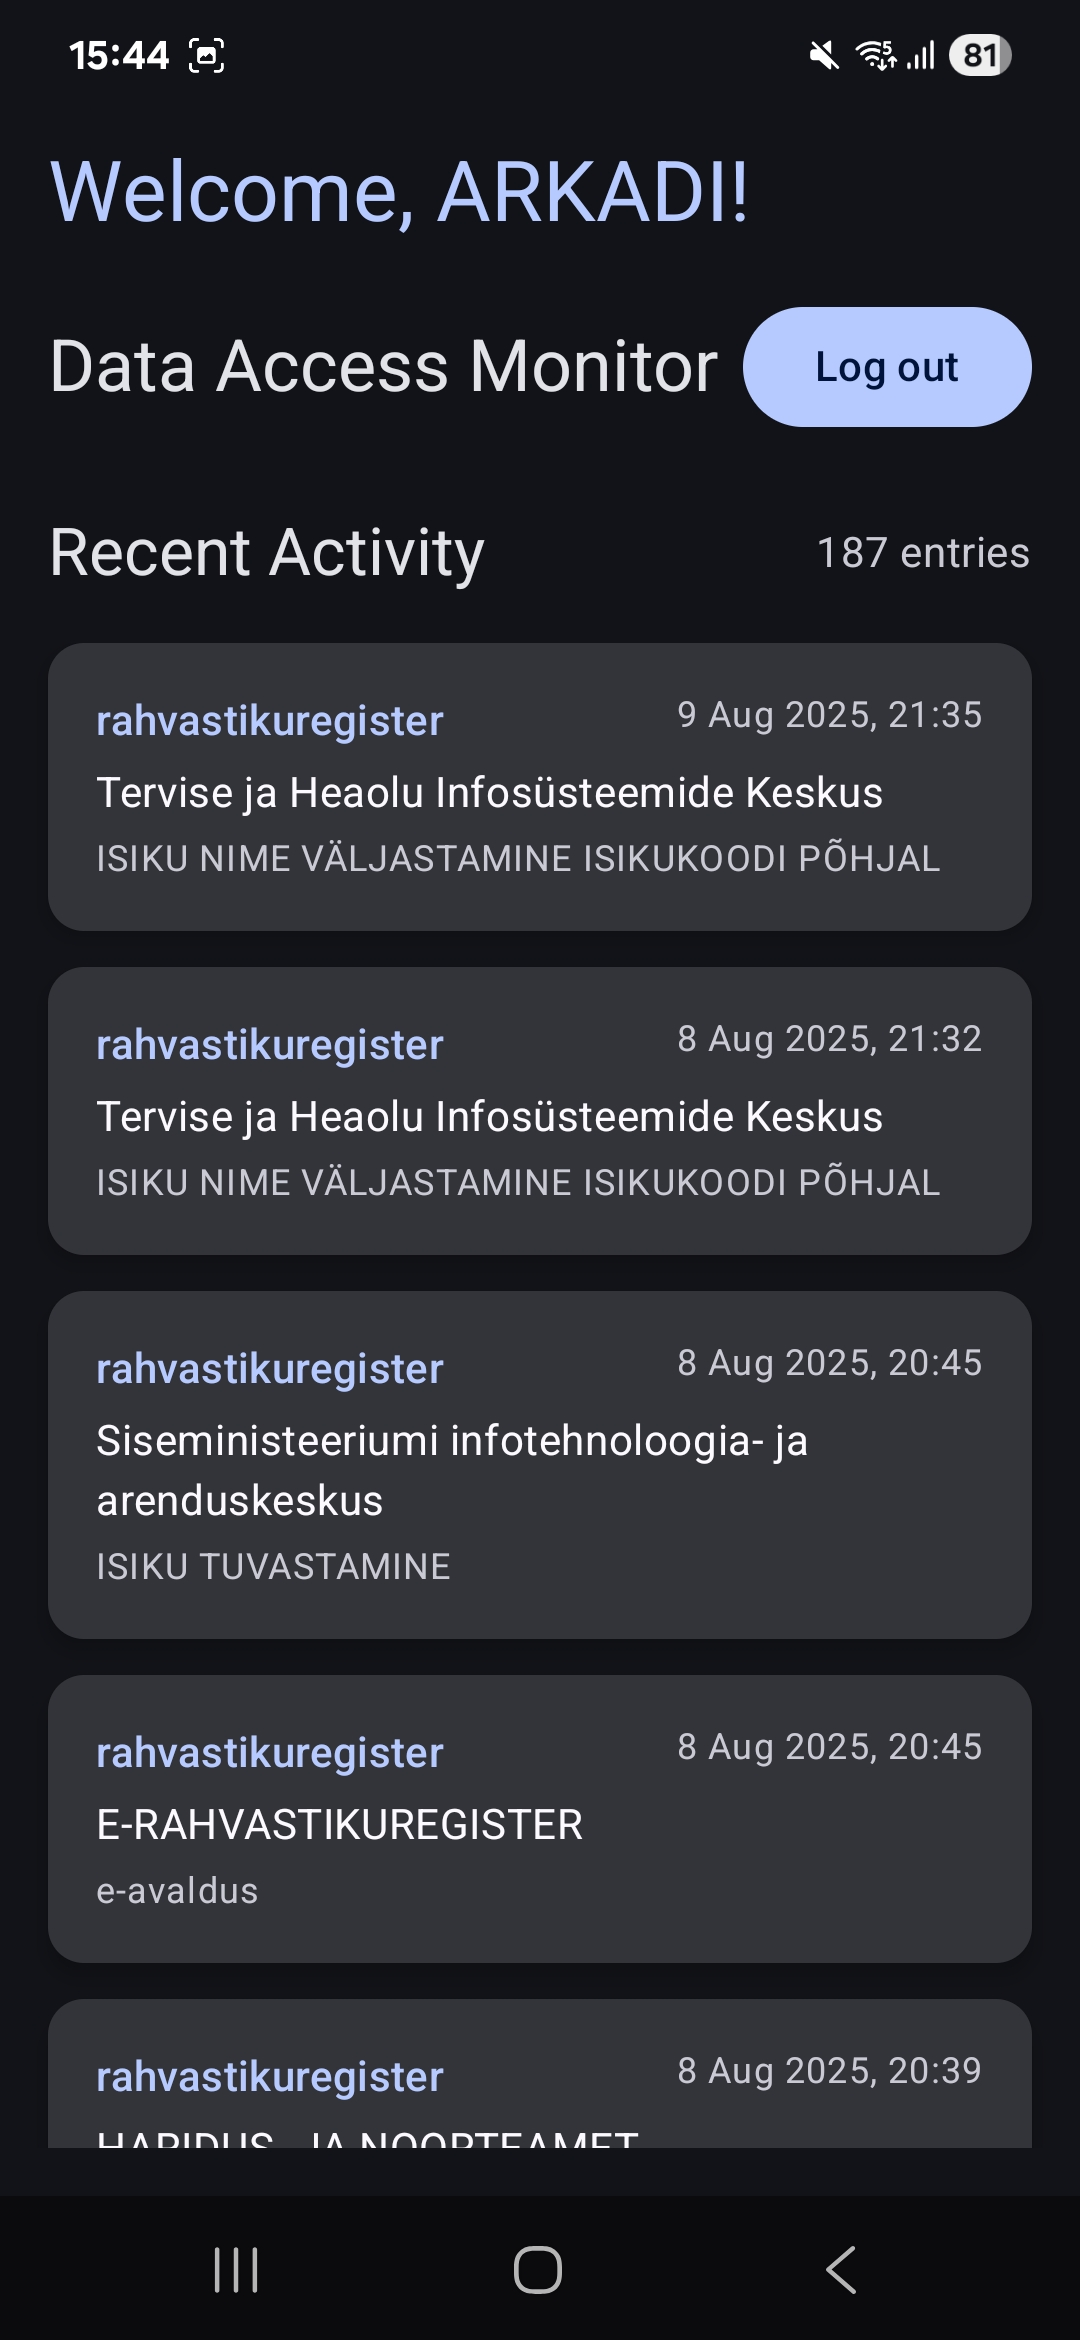
\includegraphics[width=\textwidth]{english/figures/Screenshot_20250810_154411_Data Access Notifier.jpg}
\end{minipage}
\caption{Authentication to Data Access Notifier}
\label{fig:app-usage}
\end{figure} 

\begin{figure}[H]
\centering
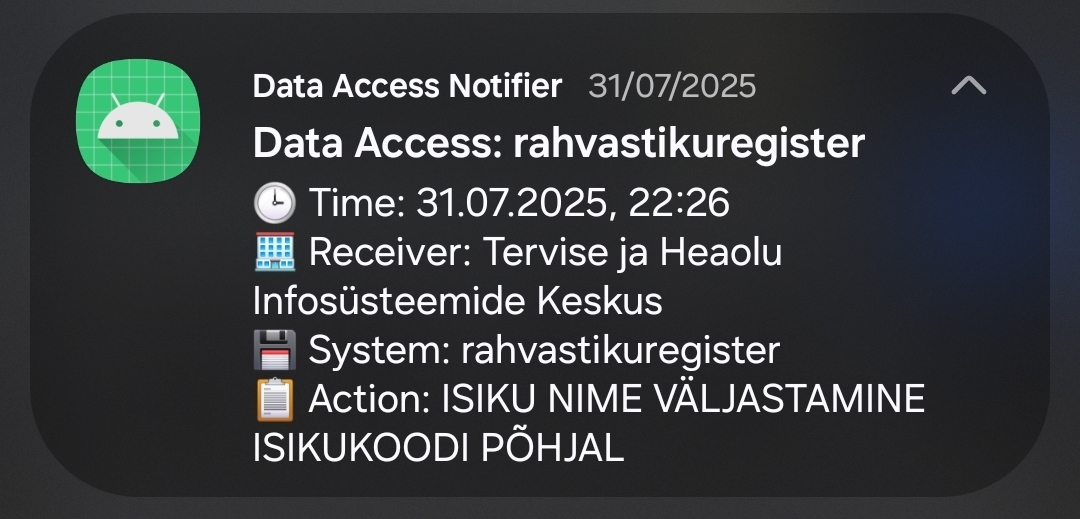
\includegraphics[width=250px]{english/figures/Screenshot_20250801_133754_Signal.jpg}
\caption{Data access notification}
\label{fig:data-access-notification}
\end{figure}

\subsection{Observations while using \textbf{Data Access Notifier}}
\label{observations}

While using the \textbf{Data Access Notifier} application over several weeks, I made several interesting observations about the behavior of the \textit{Andmejälgija} API and the reliability of real-time access logging.

One notable discovery was related to delayed log entries. I occasionally received notifications for access events dated several months in the past - specifically, events from May 2025 would sometimes appear in August 2025. Initially, I suspected this might be a deduplication issue within the application, but after examining the stored notification history, it became clear that these were genuinely new log entries that had not been seen previously by the application.

This behavior suggests that there may be delays in the centralized logging infrastructure of \textit{Andmejälgija}, where some access events are not immediately recorded or made available through the API.

The application proved to be quite reliable in maintaining the authentication session during the 12-hour window. The hybrid AlarmManager approach (described in \ref{alarmmanager-approach}) successfully maintained connectivity even during extended periods of device inactivity or network fluctuations.

From a user experience perspective, the notifications provided valuable insights into data access patterns that would otherwise remain invisible to citizens. This transparency feature proved particularly useful for understanding which organizations access personal data and how frequently such access occurs.

\subsection{Limitations}
The most significant limitation of the \textbf{Data Access Notifier} application is the 12-hour session expiry imposed by the \textit{GovSSO} authentication system. As discussed in \ref{session-limitations}, this server-side restriction cannot be circumvented through known technical means, requiring users to manually re-authenticate.

While the application successfully preserves all access log data during authentication gaps - ensuring no events are permanently lost - the periodic interruptions in real-time monitoring represent a substantial usability constraint.

Additionally, the application's scope is currently limited to Android devices running version 8.1 and higher. While this covers approximately 96.4\% of the Android ecosystem, users of iOS or other mobile platforms cannot benefit from this solution without platform-specific implementations.

The reliance on reverse-engineered internal APIs also introduces inherent fragility. Changes to \textit{eesti.ee}'s internal API structure or authentication mechanisms could potentially break the application's functionality without notice, requiring an update to the application to fix the issue.

Additionally, the session-based approach requires the device to maintain active network connectivity and remain operational to perform periodic authentication renewals and API polling. Extended periods of device inactivity, airplane mode, or network unavailability will result in session expiry and temporary loss of monitoring capabilities.

The application also doesn't currently support the access logging implemented in \textit{E-File}.

Finally, the \textit{Andmejälgija} protocol itself is not regulated by the law, and information systems are not required to implement it, and even if they do, not all data access events are guaranteed to be timely distributed or logged at all.

\subsubsection{Tested devices}
The \textbf{Data Access Notifier} application has been tested on the following devices:
\begin{itemize}
    \item Xiaomi Poco X3 Pro running CrDroid without Google Services 
    \item Xiaomi Redmi 7A running Lineage OS without Google Services
    \item Samsung Galaxy S25 with stock OS (Google Services included)
\end{itemize}

\subsection{Battery usage}
\textbf{Data Access Notifier} application maintains relatively low power consumption despite its continuous background operation. The hybrid AlarmManager approach with short-lived foreground services appears to be efficient in terms of battery impact.

While the battery utilization hasn't been actively monitored, some screenshots have been taken on Samsung Galaxy S25 at different times during the active use period.

\begin{figure}[H]
\centering
\begin{minipage}{0.32\textwidth}
    \centering
    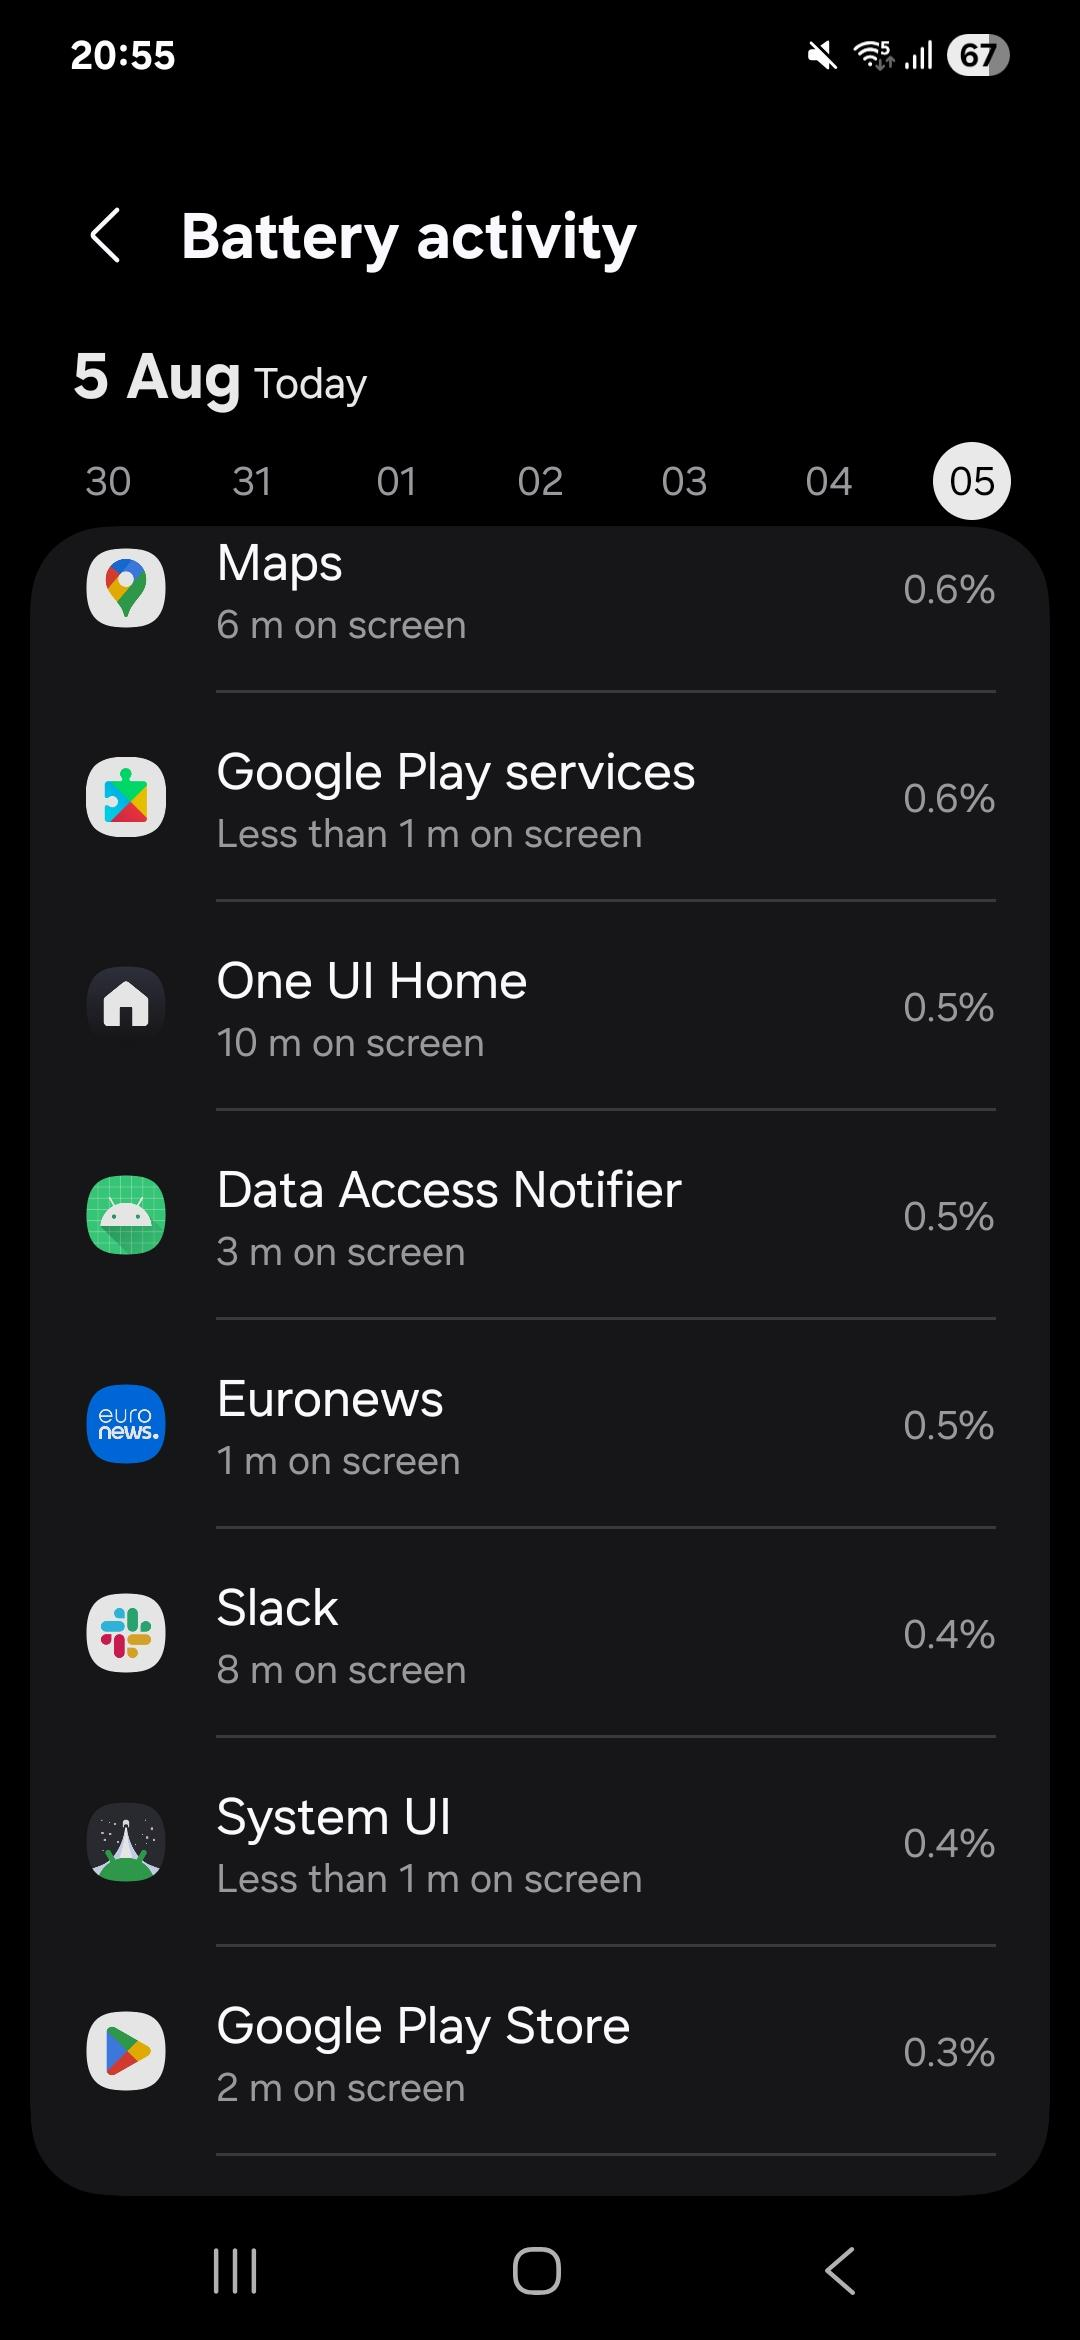
\includegraphics[width=\textwidth]{english/figures/IMG_20250809_225839_242.jpg}
\end{minipage}%
\hfill
\begin{minipage}{0.32\textwidth}
    \centering
    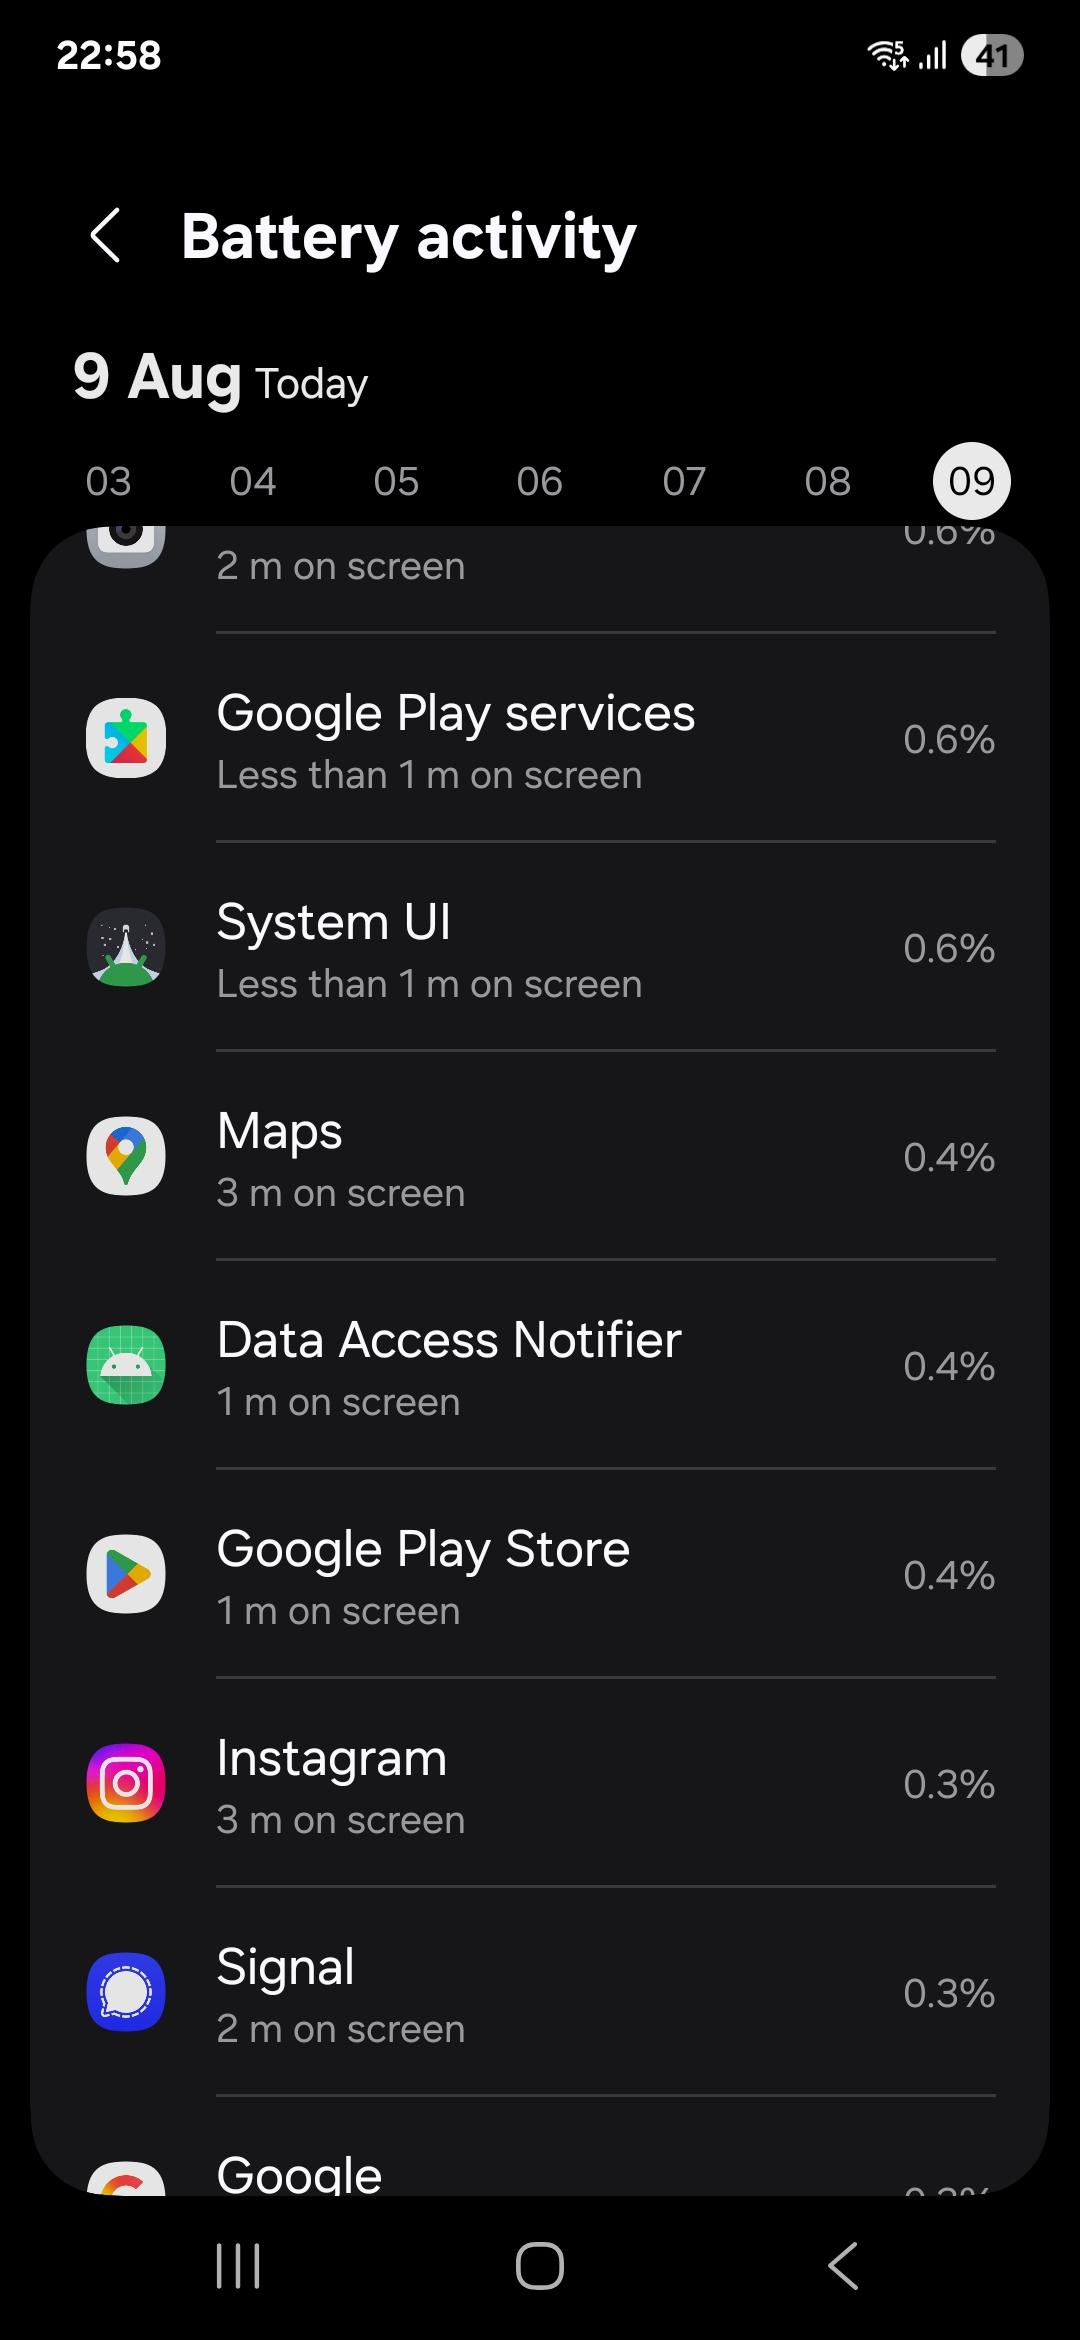
\includegraphics[width=\textwidth]{english/figures/IMG_20250809_225839_290.jpg}
\end{minipage}%
\hfill
\begin{minipage}{0.32\textwidth}
    \centering
    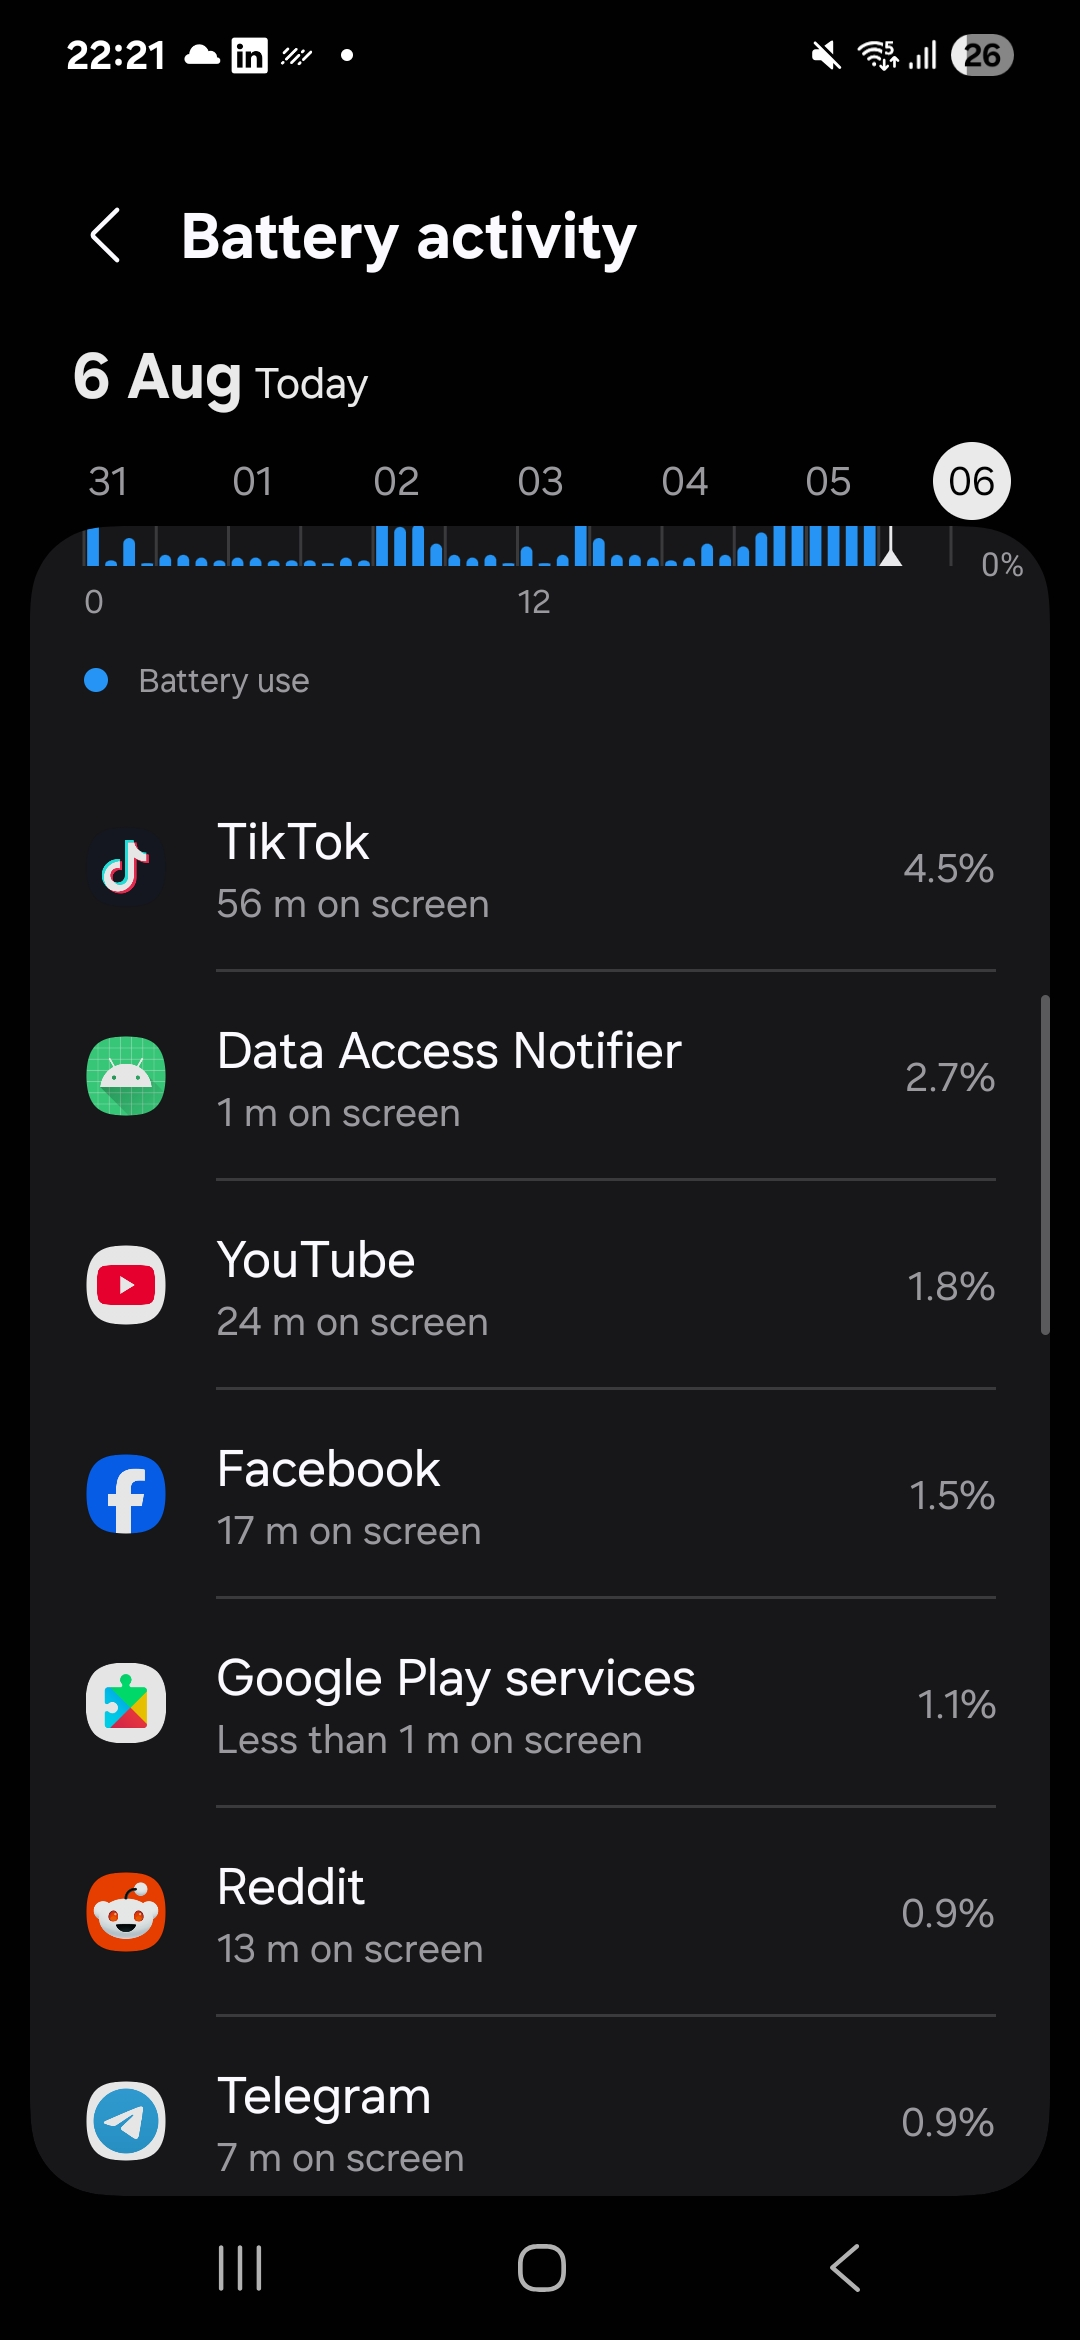
\includegraphics[width=\textwidth]{english/figures/IMG_20250809_225839_295.jpg}
\end{minipage}
\caption{Battery usage for Data Access Notifier application on Samsung Galaxy S25 showing power consumption over different time periods during active use.}
\label{fig:battery-usage}
\end{figure}

\subsection{Bug reports}

During the development and testing phases, users are encouraged to report any bugs, issues, or unexpected behavior through the GitHub Issues page of the project repository \cite{data-access-notifier}. When submitting bug reports, users should include:

\begin{itemize}
    \item Device model and Android version
    \item Detailed description of the issue
    \item Steps to reproduce the problem
    \item Any relevant error messages or screenshots
    \item Application version number
\end{itemize}

This feedback mechanism helps improve the application's stability and reliability across different Android devices and configurations.

\subsection{Contributions}
The \textbf{Data Access Notifier} project welcomes contributions from the community. Contributions are to be submitted as pull requests to the GitHub repository. Contributors can also contact the original author directly at arkadistatsenko@gmail.com for questions, suggestions, or collaboration opportunities.




